\chapter{Követelmények a játékommal szemben}
Játék tervezésénél fontos szem előtt tartani azokat a követelményeket, amelyeknek meg kell felelnie. A felhasználói élmény szorosan kapcsolódik ahhoz, hogy a játékosok mennyire értik meg a játék működését, és ezen élmény tervezése alapvető fontosságú.


\section{Felhasználói élmény kialakítása}

A felhasználói élmény kialakítása során kiemelt figyelmet kell fordítani az elrendezésre, az egyértelmű utasításokra. A játékosoknak világosan kell látniuk, hogy hogyan tudnak interakcióba lépni a játék világával, és ezek az elemek nagyban hozzájárulnak a felhasználói élmény minőségéhez.

Az érthető és könnyen kezelhető felhasználói felület kulcsfontosságú a játék sikeréhez. A játékosoknak könnyen kell tudniuk kezelni a játék funkcióit és lehetőségeit, hogy maximálisan élvezhessék a játékot.

Az is fontos tényező, hogy a játék érthetősége és használhatósága ne csak a tapasztalt játékosok számára legyen megfelelő, hanem a kezdők és a kevésbé jártas személyek számára is könnyen hozzáférhető legyen. Az egyszerű és intuitív felület tervezése segíthet abban, hogy minél több játékos élvezhesse a játékot.


\section{Grafika}

A játékok szempontjából a grafika kulcsfontosságú elem. Egy gondosan kidolgozott vizuális megjelenés mélyebben elvonja a játékosokat a játék világába, ami növeli a játék élvezetét.

Ezért fontos számomra, hogy saját magam készítsem el a rajzokat, ezzel is egyedivé téve a játékot, illetve a fejlesztés során egyszerűbben áthidalhatok majd a grafikai problémákat, hiszen nem kell harmadik féllel egyeztetnem. A pálya kirajzolásánál szeretnék megvalósítani hamis 3D-s hatást, hogy a játékosok számára élethűbbnek tűnjön a játék. 


\section{Menürendszer}

A menürendszernek általában a játékhoz illőnek kell lennie, hogy a játékosok ne érezzék azt, hogy egy másik játékot indítanak el. Fontos az is hogy átlátható legyen, hogy a játékosok könnyen eligazodjanak benne, és ne kelljen sok időt tölteniük azzal, hogy megtalálják a keresett funkciót.

\begin{figure}[H]
    \centering
    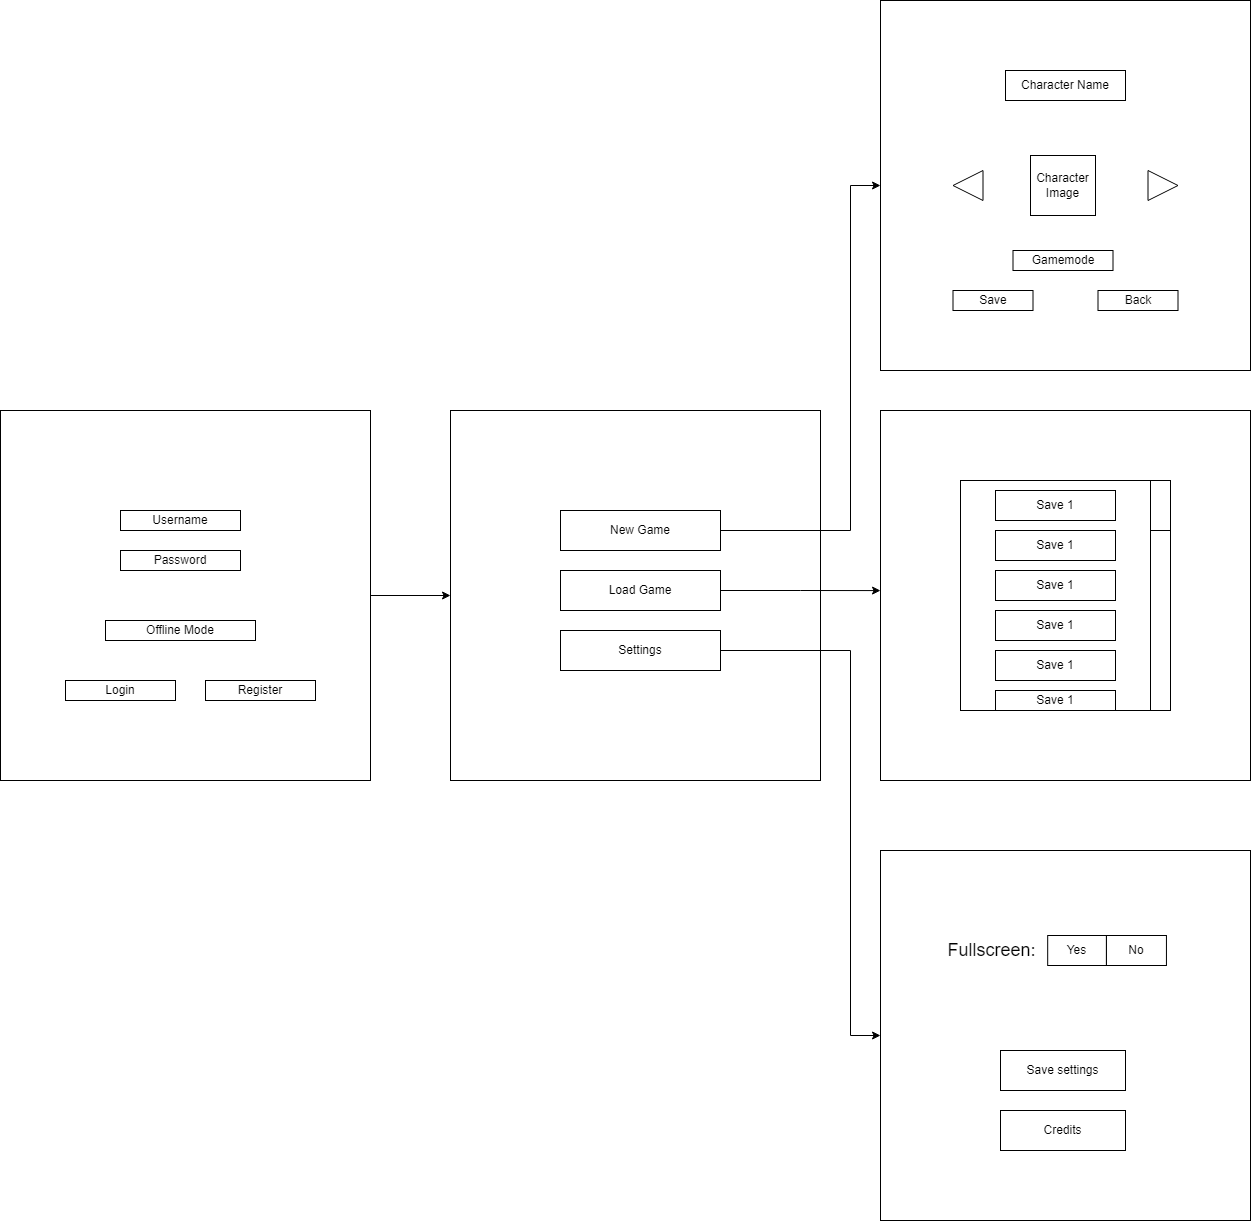
\includegraphics[width=14.0truecm]{images/MS_menu.drawio.png}
    \caption{Menürendszer terve}
    \label{fig:Menürendszer terve}
\end{figure}

\subsection{Felhasználói fiók}
Felhasználói fiók létrehozása azért szükséges a játékomban, mivel szeretnék létrehozni egy ranglista rendszert, ahol a játékosok tudnak egymással versengeni, hogy ki hányszor vitte végig a játékot anélkül, hogy a karaktere egyszer is meghalt volna, miközben a szörnyek minden újrakezdést követően erősödnek. Ehhez a rendszerhez elengedhetetlen, hogy a játékosokat megtudjam különböztetni, illetve, hogy egy adatbázisban eltudjam tárolni a játékosok adatait.

\begin{figure}[H]
    \centering
    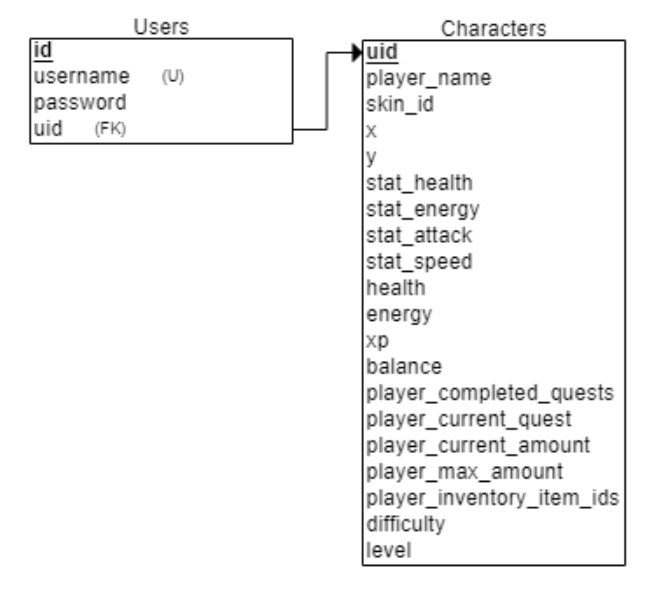
\includegraphics[width=10.0truecm]{images/RelationModell.png}
    \caption{Relációs modell}
    \label{fig:Relációs modell}
\end{figure}

\subsection{Főmenü funkciói}

A bejelentkezést követően a játékosoknak három menüpont fog elérhetővé válni. Az egyik kiemelkedően fontos lehetőség a beállítások menüpont lesz, mivel általában itt találhatók a kulcsfontosságú funkciók módosítására szolgáló lehetőségek. Az én esetemben itt lesz elérhető a teljesképernyős mód beállítása. A beállítások menüpont alatt továbbá megtalálható lesz egy "Credits" opció is, ami tartalmazni fogja a készítő nevét és az elkészítés évét. A másik két menüpontnak pedig a játék indításával kell kapcsolatosnak lennie, mivel a játékosoknak lehetőségük lesz új karakter létrehozására, illetve meglévő mentésük betöltésére.


\subsection{Játékon belüli menürendszer}

A legtöbb játékban kiemelkedő jelentőségű a játékon belüli pillanatálj funkció, valamint egy belső menürendszer. Lényeges, hogy ezek könnyen elérhetőek legyenek, miközben nem zavarják a játékélményt. A játékosoknak lehetőségük lesz a játék közben is hozzáférni egy beállítások menühöz, amelyben a hangerőszintet is be tudják majd állítani. Ezen menü részét kell képeznie egy mentés funkciónak, ami a játék aktuális állapotának mentését teszi lehetővé, továbbá egy folytatás lehetőségnek, és egy kilépés opciónak, amely a játék bezárását szolgálja.


\section{Felhasználói felület és a játékos cselekvési lehetőségei}

A játékokban fontos a jól megtervezett felhasználói felület, amely lehetővé teszi a játékosok számára, hogy a lehető legkönyebben és leggyorsabban elérjék a kívánt funkciókat. Ilyen felület a HUD (Head Up Display)  ez segíti a játékosokat abban, hogy valós idejű információkkal rendelkezzenek a játék világáról, így gyorsabban és hatékonyabban reagálhatnak a különböző helyzetekre.


\subsection{Felhasználói felület}

A felhasználói felület megtervezése során, igyekeztem figyelni, a letisztultságra és a felhasználói élményre. Fontosnak tartottam, hogy a design egyszerű és könnyen átlátható legyen, hogy a felhasználó könnyedén megtalálja azokat a funkciókat és információkat, amelyekre szüksége van.

A HUD (Head Up Display) a játék során folyamatosan látható lesz, így a játékosoknak nem kell külön menübe navigálniuk, hogy megtalálják a szükséges információkat. A HUD a játékos karakterének életpontjait, energia szintjét, a játékos aranyát, a játékos szintjét, a játékos tapasztalati pontjait, a játékos fegyverét, a játékos által használt italokat fogja megjeleníteni.

\begin{figure}[H]
    \centering
    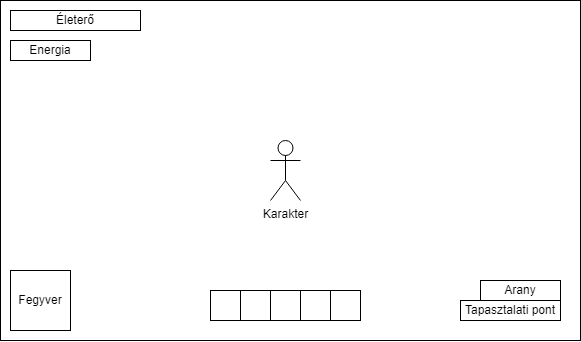
\includegraphics[width=14.0truecm]{images/MS_UI.drawio.png}
    \caption{Felhasználói felület terve}
    \label{fig:Felhasználói felület}
\end{figure}

\subsection{Életpontok és Energia}

A játékos karakterének életpontjai mutatják meg, hogy mennyi sebzést tudnak még elszenvedni mielőtt meghalna a karakterük. Az energia szint pedig a karakter futásához és cselekvéseihez szükséges energiaforrás. A megfelelő kezelése és felhasználása kulcsfontosságú a túléléshez és a harc hatékonyságához.

\subsection{Fegyver Választás}

A játékosnak lehetősége van különböző fegyverek között választani, amelyek különböző képességekkel és támadási stílusokkal rendelkeznek. Ez lehetővé teszi számára, hogy testre szabja a harci stratégiáját és alkalmazkodjon az adott helyzethez.

\subsection{Harcolás Szörnyekkel}

A játék során a játékosnak számos szörnnyel kell megküzdenie. A harcok izgalmasak és változatosak, és a játékosnak ki kell használnia a karaktere készségeit és fegyvereit a sikeres küzdelem érdekében. A szörnyek legyőzése tapasztalati pontokat és esetleges zsákmányt is eredményez.

\subsection{Küldetések Felvétele}

A lineáris történetvezetés lehetőséget kínál arra, hogy a játékosok fokozatosan mélyüljenek el a játék világában, miközben követik a fő cselekményt. A küldetések integrálása a lineáris narratívába lehetővé teszi, hogy a játékosok szorosan kövessék a történet fő vonalát, miközben változatos kihívásokkal találkoznak.

A küldetések kiváló lehetőséget nyújtanak a karakterfejlődésre és a történet gazdagítására. Az XP (tapasztalati pont) és jutalmak rendszere ösztönzi a játékosokat, hogy aktívan részt vegyenek a küldetésekben, és ezáltal fokozatosan erősödjenek a játékban. A lineáris elbeszélésmód segítségével a küldetések sorrendje és nehézségi szintje könnyen szabályozható, így biztosítható a folyamatos kihívás és az érdekesség fenntartása.

\subsection{Italok Vásárlása és Használata}

A játékos aranyat szerezhet a játék során, amit italokra is fordíthat. Az italok különböző hatásokkal rendelkeznek, például életpont visszatöltés vagy energia szint növelés. Az italok stratégiai használata a túlélés és a harcok kulcsa lehet.

\subsection{Statisztikák Növelése tapasztalati pontokból}

A játékos karaktere tapasztalati pontokat szerez a harcok és küldetések során. Az XP felhasználható a karakter statisztikáinak növelésére, például az erő, az ügyesség vagy a mágia terén. Ez lehetővé teszi a karakter fejlődését és a játékmenet testreszabását.

Ezen cselekvési lehetőségek összekapcsolva teremtenek egy gazdag és dinamikus játékélményt az Action RPG játékban, ahol a játékos döntései és cselekedetei hatással vannak a karakter fejlődésére és a játék világára.



